% !TEX root = ../main.tex

\begin{figure}[htbp]
  \centering
  \vspace*{-0.75\baselineskip}
  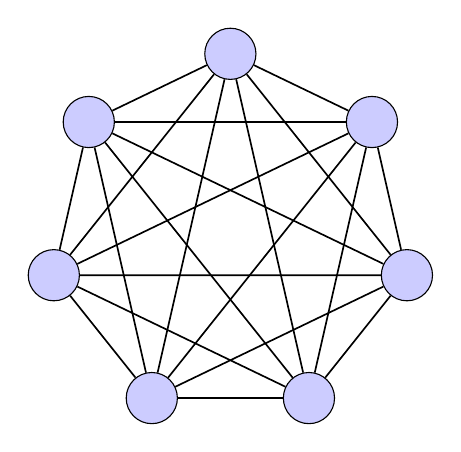
\begin{tikzpicture}[
    scale=1.0,
    every node/.style={transform shape},
    v/.style={circle, draw, fill=blue!20, minimum size=6.5mm, inner sep=0pt, font=\small},
    e/.style={draw, line width=0.6pt}
  ]
    % K7 (grafo completo con 7 vértices)
    \def\N{7}
    \def\R{2.3}

    % Vértices en un círculo
    \foreach \i in {1,...,\N} {
      \node[v] (v\i) at ({90 - 360*(\i-1)/\N}:\R) {};
    }

    % Aristas completas (i < j)
    \foreach \i in {1,...,\N} {
      \foreach \j in {\i,...,\N} {
        \ifnum\i<\j
          \draw[e] (v\i) -- (v\j);
        \fi
      }
    }
  \end{tikzpicture}
  \caption{Grafo completo $K_7$.}
  \label{fig:k7}
\end{figure}

